\documentclass[tikz]{standalone}
\usepackage{pgfplots}
\pgfplotsset{compat=1.18}
\begin{document}
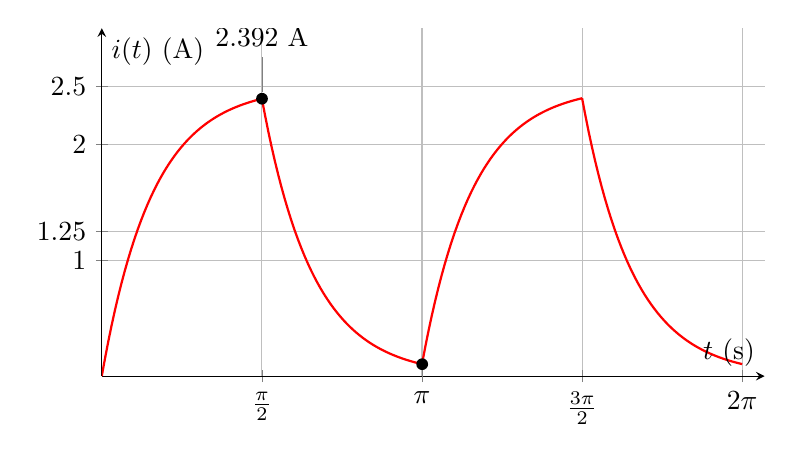
\begin{tikzpicture}
\begin{axis}[
    axis lines = middle,
    xlabel = {$t$ (s)},
    ylabel = {$i(t)$ (A)},
    xmin = 0, xmax = 6.5,
    ymin = 0, ymax = 3,
    xtick = {0, 1.57, 3.14, 4.71, 6.28},
    xticklabels = {0, $\frac{\pi}{2}$, $\pi$, $\frac{3\pi}{2}$, $2\pi$},
    ytick = {0, 1, 1.25, 2, 2.5},
    grid = both,
    width=10cm, height=6cm
]
% Cycle 1: 0 to pi/2 (Square wave is high at 10V)
\addplot[red, thick, domain=0:1.57, samples=50] {2.5*(1 - exp(-2*x))};
% Cycle 1: pi/2 to pi (Square wave is low at 0V)
\addplot[red, thick, domain=1.57:3.14, samples=50] {2.392*exp(-2*(x-1.57))};

% Cycle 2: pi to 3pi/2
\addplot[red, thick, domain=3.14:4.71, samples=50] {2.5 - (2.5 - 0.1034)*exp(-2*(x-3.14))};
% Cycle 2: 3pi/2 to 2pi
\addplot[red, thick, domain=4.71:6.28, samples=50] {2.396*exp(-2*(x-4.71))};

% Labels
\node[circle, fill, inner sep=1.5pt, pin=90:{2.392 A}] at (axis cs:1.571, 2.392) {};
\node[circle, fill, inner sep=1.5pt, pin=-90:{0.103 A}] at (axis cs:3.142, 0.103) {};

\end{axis}
\end{tikzpicture}
\end{document}
